%!TEX program = xelatex
%!BIB program = bibtex
\documentclass[cn,black,12pt,normal]{elegantnote}
\usepackage{float}
\usepackage{hyperref}
\usepackage{amsmath}
\usepackage{amsfonts}
\usepackage{amssymb}
\usepackage{siunitx}[=v2]
\usepackage{fancyhdr}
\usepackage{newtxtext}
\usepackage{algorithm}
\usepackage{algorithmic}
\newcommand{\uct}[1]{\textsuperscript{\textsuperscript{\cite{#1}}}}
\renewcommand{\tablename}{\textbf{Table}}
\renewcommand{\figurename}{Figure.}
\renewcommand{\refname}{References}
\renewcommand{\contentsname}{Contents}
\renewcommand{\versiontext}{Version: }
\renewcommand{\updatetext}{Update: }
\PassOptionsToPackage{no-math}{fontspec}
\lstset{basicstyle=\footnotesize\ttfamily\color[RGB]{50,0,130},numbers=none,frame=trBL}

\sisetup{mode=text}
\sisetup{range-phrase = \text{ \textasciitilde }}
\pagestyle{fancy}
\fancyhead[L]{School of Software Engineering, Tongji University}
\fancyhead[R]{Data Structure Projects}
\renewcommand{\headrulewidth}{1pt}

\title{Josephus problem\\约瑟夫生者死者游戏}
\author{1951510\; 姜文渊}
\institute{\small \url{https://github.com/jwyjohn/Jwy_DataStructureHomework}}
\version{0.50}
\date{\today}

\begin{document}

\maketitle

\textbf{Data structure involved:} Singly circular linked list


\tableofcontents

\newpage


\section{Introduction}

The well-known Josephus problem is described as follows:

People are standing in a circle waiting to be executed. Counting begins at a specified point in the circle and proceeds around the circle in a specified direction. After a specified number of people are skipped, the next person is executed. The procedure is repeated with the remaining people, starting with the next person, going in the same direction and skipping the same number of people, until certain number of people remain.\uct{wiki:Josephus_problem}

The problem is named after Flavius Josephus, a Jewish historian living in the 1st century. According to Josephus' account of the siege of Yodfat, he and his 40 soldiers were trapped in a cave by Roman soldiers. They chose suicide over capture, and settled on a certain serial method of committing suicide.\uct{wiki:Josephus_problem}

The Josephus problem is a theoretical problem studied in computer science and mathematics which relates to a certain counting-out game. Simple as it may seem to be, the generalized form of this problem leads to many interesting findings. The most well studied case is to kill every 2 people. When it comes to kill every 3 people, until 1997, Lorenz Halbeisen and Norbert Hungerbühler gave out a closed-form formula to slove this case.

In this project, the author built a demo for simulating the Josephus problem with $n$ people numbered from $1$ to $n$, starting from position $s$, kill one every $k$ people and left $m$ people ($n\geq s,m >0$,$k>0$), using Singly circular linked list.

Another version of this problem comes from a historic tale which involves 15 Turks and 15 Christians aboard a ship in a storm which will sink unless half the passengers are thrown overboard. All 30 stand in a circle and every ninth person is to be tossed into the sea. The Christians need to determine where to stand to ensure that only the Turks are tossed.\uct{newman1988world}

This is the case where $n=30$, $s=1$, $k=9$ and $m=15$, which will be calculated in the demo below.

\section{Demostration}

\subsection{Compile and run the program}

On linux platform with \lstinline{make} and a \lstinline{g++} which supports C++ 11 Standard, just \lstinline{cd} to the \lstinline{./linux} and run \lstinline{make build}. The binary executable will be generated in the same dirctory named as \lstinline{a.out} or \lstinline{exam}, according to the configurations in the \lstinline{Makefile}. Use \lstinline{./a.out} or \lstinline{./joseph}to run the program.

The program is an interactive shell, where you can input commands and get results.

\begin{figure}[H]
    \centering
    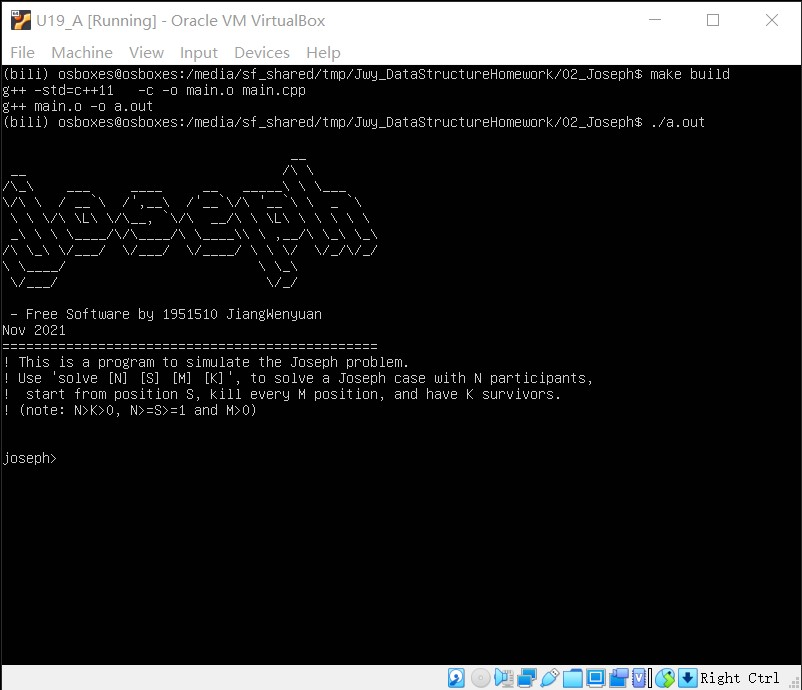
\includegraphics[width=0.7\linewidth]{image/j01.jpg}
    \caption{The user interface of the program}
\end{figure}

Usage of commands can be found on the main screen, and the \lstinline{help} command can give you information about theses commands.  All available commands is listed below.

\begin{enumerate}
    \item \lstinline{help} : Show help for a certain command.
    \item \lstinline{exit} : Exit the program.
    \item \lstinline{solve [N] [S] [K] [M]} : Simulate the Josephus problem with $n$ people numbered from $1$ to $n$, starting from position $s$, kill one every $k$ people and left $m$ people ($n\geq s,m >0$,$k>0$).
\end{enumerate}
Note that if a user inputs invalid commands or arguments, the program will be robust enough (at least to some extent) to detect the exception and return an error message. Detailed Demostration of this feature can be explored when using this program.
\subsection{Solve some cases}

\paragraph{Case 1} Type \lstinline{solve 30 1 9 15} . Then the killed people and the survivors will be shown.

\begin{figure}[H]
    \centering
    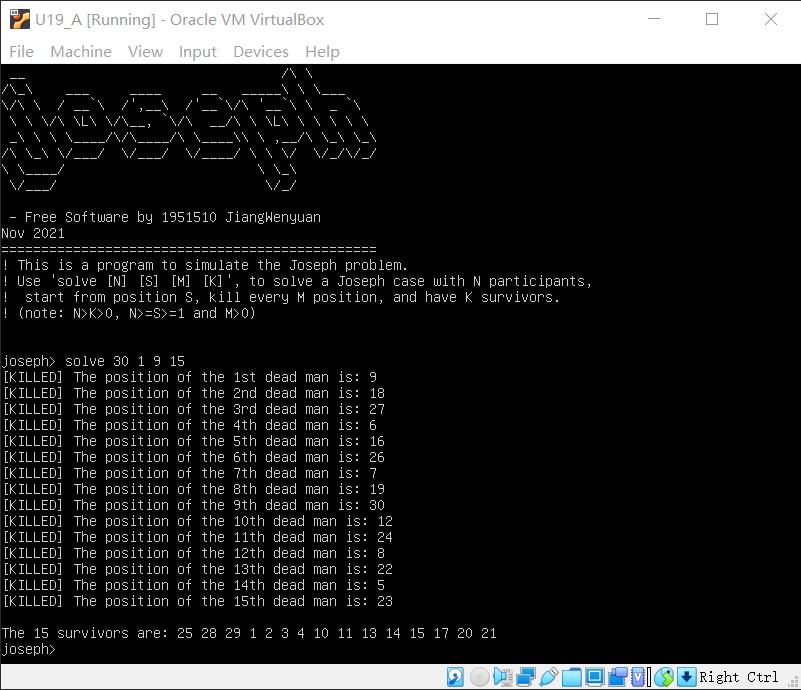
\includegraphics[width=0.7\linewidth]{image/j02.jpg}
    \caption{The result of case \lstinline{solve 30 1 9 15}}
\end{figure}

\paragraph{Case 2} Type \lstinline{solve 30 1 9 1} . Then the killed people and the survivors will be shown.

\begin{figure}[H]
    \centering
    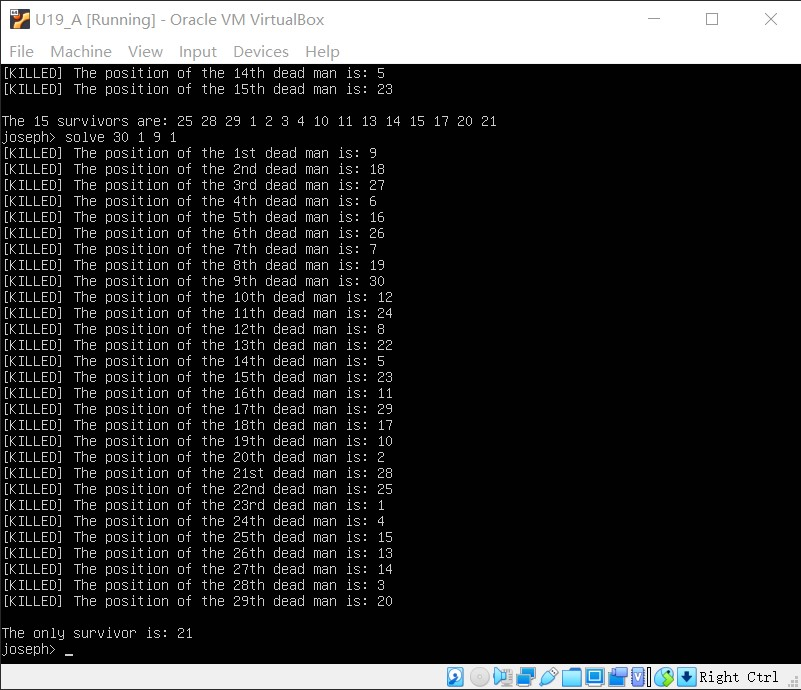
\includegraphics[width=0.7\linewidth]{image/j03.jpg}
    \caption{The result of case \lstinline{solve 30 1 9 1}}
\end{figure}

\paragraph{Case 2} Type \lstinline{solve 30 1 2 1} . Then the killed people and the survivors will be shown.

\begin{figure}[H]
    \centering
    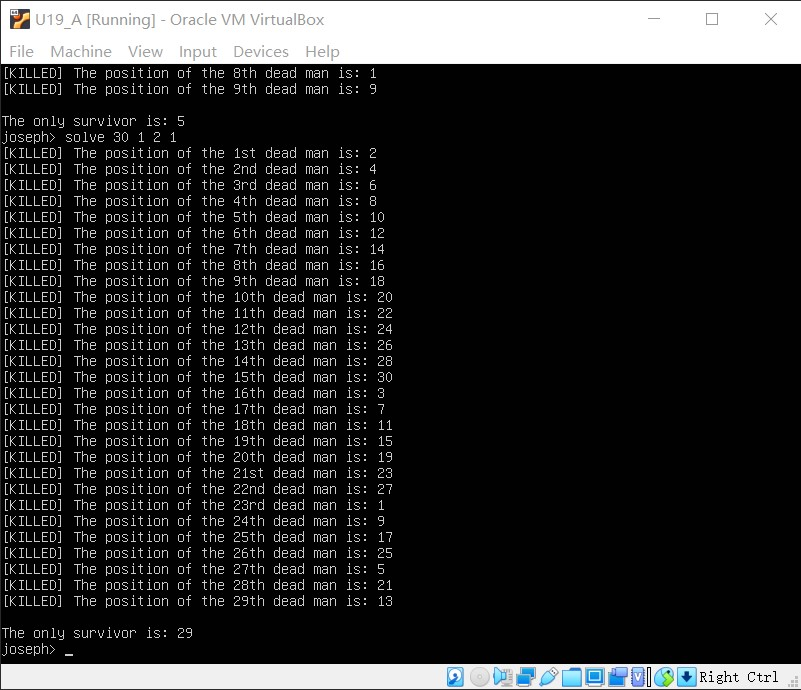
\includegraphics[width=0.7\linewidth]{image/j04.jpg}
    \caption{The result of case \lstinline{solve 30 1 2 1}}
\end{figure}

\section{About linked list}

Linked list is a data structure consisting of a collection of nodes with pointers onto their next node, which together represent a sequence. A simple figure below can demostrate the basic features of a linked list. \uct{wiki:Linked_list}

\begin{figure}[H]
    \centering
    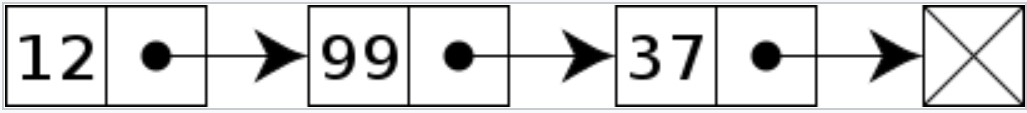
\includegraphics[width=1.0\linewidth]{image/ll_01.jpg}
    \caption{A simple diagram showing a \textbf{Singly linked list} (diagram produced by Lasindi)}
\end{figure}

There are several improvements on this data structure. A well-known variant of the Singly linked list is the \textbf{Circular linked list}, whose 'last' node points to its 'first' node, as is shown in the figure below.

\begin{figure}[H]
    \centering
    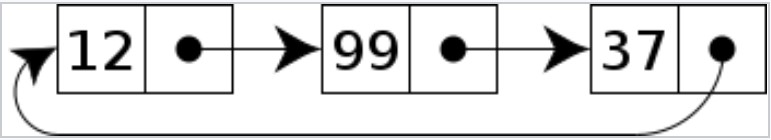
\includegraphics[width=1.0\linewidth]{image/ll_03.jpg}
    \caption{A simple diagram showing a \textbf{Circular linked list} (diagram produced by Lasindi)\uct{wiki:Linked_list}}
\end{figure}


There are many other ways to implement a circular structure, for example, we could combine modular arithmetic with common linear data structures like array to build a circular data structure. Compared with many other data structures, the Circular linked list had an advantage that it can insert and delete an element in a circular structure with less effort. However, to find an element in a Circular linked list, the time cost is the same as linked list, which is $O(n)$.


\section{Notes on the source code}

If you want to modify or re-use the author's code, here are some explaination about the important part of the code. Comments in the source file can provide detailed help, but the following shows the outline.

The node of a linked used in this project is defined here:
\begin{lstlisting}[language = C++]
struct exam_candidate
{
    struct node
    {
        int no;
        node *next;
    };
    
};
\end{lstlisting}
which is a singly linked list with \lstinline{*next} pointer.

There are two global pointers:
\begin{lstlisting}[language = C++]
node *current;
node *pre;
\end{lstlisting}
The \lstinline{current} points to the node that is currently being processed, while the \lstinline{pre} is the precedent node of the current node. The \lstinline{pre} is of much importance, since the operations involve changing the \lstinline{node *next;} of the precedent node.

To initialize the $n$ people circle, the \lstinline{int init()} is called.
\begin{lstlisting}[language = C++]
int init()
{
	current = new node;
	node *first = current;
	for (int i = 1; i < N; i++)
	{
		current->no = i;
		current->next = new node;
		current = current->next;
	};
	current->no = N;
	current->next = first;
	pre = current;
	while (pre->next->no != S)
	{
		pre = pre->next;
	};
	current = pre->next;
	return 0;
};
\end{lstlisting}
As you can see, \lstinline{current->next = first;} makes the linked list circular, and the following code adjusts the \lstinline{current} and \lstinline{pre} to point to correct element.

The solving process is coded in \lstinline{int solve()}. The most important part is the while loop shown below.
\begin{lstlisting}[language = C++]
int solve()
{
......
	while (count > K)
	{
		for (int i = 0; i < M - 1; i++)
		{
			current = current->next;
			pre = pre->next;
		};
		if (j % 10 == 1 && j != 11)
			ch = "st";
		else if (j % 10 == 2 && j != 12)
			ch = "nd";
		else if (j % 10 == 3 && j != 13)
			ch = "rd";
		else
			ch = "th";
		cout << "[KILLED] The position of the " << j << ch << " dead man is: " << current->no << endl;
		j++;
		pre->next = current->next;
		delete current;
		current = pre->next;
		count--;
	};
......
	return 0;
};
\end{lstlisting}
The \lstinline{for (int i = 0; i < M - 1; i++)} loop finds the person to kill, and updates the \lstinline{current} and \lstinline{pre} pointer. When the \lstinline{current} and \lstinline{pre} are well set, we remove the \lstinline{current} node using the classical way:
\begin{lstlisting}[language = C++]
int solve()
{
......
......
		pre->next = current->next;
		delete current;
		current = pre->next;
		count--;
	};
......
	return 0;
};
\end{lstlisting}
In this code block, you will find that the \lstinline{pre} pointer is necessary for the removal of the current node. After the \lstinline{while (count > K)} loop, the elements remained in the circular linked list are the number of survivors.

The output process is also in \lstinline{int solve()}, and is shown below:
\begin{lstlisting}[language = C++]
int solve()
{
......
	{
......
		if (j % 10 == 1 && j != 11)
			ch = "st";
		else if (j % 10 == 2 && j != 12)
			ch = "nd";
		else if (j % 10 == 3 && j != 13)
			ch = "rd";
		else
			ch = "th";
		cout << "[KILLED] The position of the " << j << ch << " dead man is: " << current->no << endl;
......
	};
	cout << endl;
	if (K != 1)
	{
		cout << "The " << K << " survivors are: ";
	}
	else
	{
		cout << "The only survivor is: ";
	};
	node *stop = current;
	while (current->next != stop)
	{
		cout << current->no << " ";
		current = current->next;
	};
	cout << current->no << " ";
	cout << endl;
	return 0;
};
\end{lstlisting}

Note that most of the code in \lstinline{main.cpp} is for processing the user's input, which is not so interesting.

\section{Discussion}

Even though the performance of circular linked list is not excellent, it is a convenient way of simulating the Josephus problem. The computational complexity of the method is $O(n^2)$.

A more effective way of finding the survivors of Josephus problem is Dynamic programming, by performing the first step and then using the solution of the remaining problem. When the index starts from one, then the person at $s$ shifts from the first person is in position ${\displaystyle ((s-1){\bmod {n}})+1}$, where $n$ is the total number of persons.

Let ${\displaystyle f(n,k)}$ denote the position of the survivor. The equation for ${\displaystyle f(n,k)}$ is:
$${\displaystyle f(n,k)={\begin{cases}0&{\text{if }}n=1\\(f(n-1,k)+k){\bmod {n}}&{\text{if }}1<n<k\\\left\lfloor {\frac {k((f(n',k)-n{\bmod {k}}){\bmod {n}}')}{k-1}}\right\rfloor {\text{where }}n'=n-\left\lfloor {\frac {n}{k}}\right\rfloor &{\text{if }}k\leq n\\\end{cases}}}$$

Consider killing k-th, 2k-th, ..., ${\displaystyle (\lfloor n/k\rfloor k)}$-th people as one step, and then change the numbering. Thus this algorithm has a computational complexity of ${\displaystyle O(k\log n)}$, which is much faster than simulating the case with circular linked list.\uct{wiki:Josephus_problem}

\bibliography{references}
\end{document}
